\subsubsection{Vzájemná poloha přímek zadaných obecnými rovnicemi}
\label{subsubsec:Relative_position_general_lines}

U přímek zadaných obecnými rovnicemi můžeme jejich vzájemnou polohu
určovat pomocí normálových vektorů, které získáme přímo z koeficientů
u proměnných $x$ a $y$. V případě různoběžných přímek jejich průsečík
určíme řešením soustavy obou rovnic.

Uvažujme přímky
\[
    p:X=A+t\vec{u},
    \qquad
    q:X=B+s\vec{v},
    \qquad
    t,s\in\mathbb{R}.
\]

Uvažujme přímky
\begin{align}
    p &: a_1x+b_1y+c_1=0,
    \label{eq:General_line_p_relative_position}\\
    q &: a_2x+b_2y+c_2=0.
    \label{eq:General_line_q_relative_position}
\end{align}
Jejich normálové vektory jsou
\[
    \vec{n}_p=(a_1;b_1),
    \qquad
    \vec{n}_q=(a_2;b_2).
\]

Vzájemnou polohu přímek můžeme určit porovnáním jejich normálových
vektorů. Směrový vektor je s příslušnou přímkou rovnoběžný, zatímco
normálový vektor je k ní kolmý. Geometrický vztah mezi směrovými
a normálovými vektory obou přímek je znázorněn na obrázku
\ref{fig:Direction_normal_vectors_lines}.

Protože pootočením obou směrů o $90^\circ$ se jejich vzájemná
rovnoběžnost nezmění, platí
\[
    \vec{u}_p\parallel\vec{u}_q
    \quad\Longleftrightarrow\quad
    \vec{n}_p\parallel\vec{n}_q.
\]

Jestliže normálové vektory přímek nejsou rovnoběžné, nejsou rovnoběžné
ani jejich směrové vektory. Přímky proto mají různé směry a v rovině
se protínají právě v jednom bodě. Jsou tedy různoběžné podle definice
\ref{def:Intersecting_lines_plane}. Taková situace je znázorněna
na obrázku \ref{fig:Direction_normal_vectors_lines}.

Jestliže jsou naopak normálové vektory rovnoběžné, mají přímky stejný
směr. V takovém případě mohou být přímky buď rovnoběžné, nebo totožné.
K rozlišení těchto dvou možností již nestačí porovnat pouze koeficienty
$a_1$, $b_1$, $a_2$ a $b_2$, ale musíme porovnat všechny tři
koeficienty jejich obecných rovnic.

\begin{figure}[H]
    \centering
    \begin{tikzpicture}[scale=0.8]
       
        % Osy
        \draw[<->, thin]
            (-7,0) -- (4,0)
            node[right] {$x$};

        \draw[<->, thin]
            (0,-3) -- (0,5)
            node[above] {$y$};

        % Číselné hodnoty na ose x
        \foreach \x in {-6,-5,...,-1,1,2,...,4}
        {
            \draw (\x,0.08) -- (\x,-0.08);
            \node[below, font=\scriptsize] at (\x,0) {$\x$};
        }

        % Číselné hodnoty na ose y
        \foreach \y in {-3,-2,-1,1,2,...,4}
        {
            \draw (0.08,\y) -- (-0.08,\y);
            \node[left, font=\scriptsize] at (0,\y) {$\y$};
        }

        % Počátek soustavy
        \node[below left, font=\scriptsize] at (0,0) {$O$};

        % -------------------------------------------------
        % Přímka r_1: 2x - 3y + 6 = 0
        % tedy y = 2/3 x + 2
        % -------------------------------------------------

        \draw[thick, <->] (-6,-2) -- (3,4)
            node[pos=0.02, below right, black] {$p$};

        % -------------------------------------------------
        % Přímka r_2: x + 2y + 2 = 0
        % tedy y = -1/2 x - 1
        % -------------------------------------------------

        \draw[thick,<->] (-6,2) -- (2,-2)
            node[pos=0.02, below left, black] {$q$};

        % -------------------------------------------------
        % Směrový a normálový vektor přímky p
        % -------------------------------------------------

        % Společný počáteční bod
        \coordinate (C) at (-0.78,1.48);

        % Směrový vektor u_p
        \draw[vector] (C) -- (1.51385,3.00923)
            node[midway, below, sloped] {$\vec{u}_p$};

        % Normálový vektor n_p
        \draw[vector] (C) -- (-2.30923,3.77385)
            node[midway, right] {$\vec{n}_p$};

        % Ručně nakreslená značka pravého úhlu
        \draw (-0.558,1.628) -- (-0.706,1.850) -- (-0.928,1.702);

        % -------------------------------------------------
        % Směrový a normálový vektor přímky q
        % -------------------------------------------------

        % Společný počáteční bod
        \coordinate (F) at (-4.992,1.496);

        % Směrový vektor w
        \draw[vector] (F) -- (-3,0.5)
            node[midway, above, sloped] {$\vec{u}_q$};

        % Normálový vektor b
        \draw[vector] (F) -- (-3.996,3.488)
            node[midway, left] {$\vec{n}_q$};

        % Ručně nakreslená značka pravého úhlu
        \draw (-4.724,1.362) -- (-4.590,1.630) -- (-4.858,1.764);

    \end{tikzpicture}

    \caption{Směrové a normálové vektory různoběžných přímek $p$ a $q$.}
    \label{fig:Direction_normal_vectors_lines}
\end{figure}

Celý postup můžeme shrnout následovně:
\[
\begin{array}{c|c}
\text{Podmínka}
&
\text{Vzájemná poloha přímek}
\\
\hline
(a_2;b_2)\neq k(a_1;b_1)
&
\text{přímky jsou různoběžné}
\\[1mm]
(a_2;b_2)=k(a_1;b_1),\ (a_2;b_2;c_2)\neq k(a_1;b_1;c_1)
&
\text{přímky jsou rovnoběžné}
\\[1mm]
(a_2;b_2;c_2)=k(a_1;b_1;c_1)
&
\text{přímky jsou totožné}
\end{array}
\]
kde $k\in\mathbb{R}\setminus\{0\}$.

Prakticky můžeme rovnoběžnost normálových vektorů ověřit také pomocí vztahu,
což vychází z důlesku ze vztahu pro skalární součin (viz poznámka \ref{rem:Fast_orthogonal_vector})
\begin{equation}\label{eq:Parallel_general_lines_condition}
    a_1b_2-a_2b_1=0.
\end{equation}
Jestliže levá strana není rovna nule, normálové vektory nejsou
rovnoběžné a přímky jsou různoběžné.

\begin{figure}[H]
    \centering
    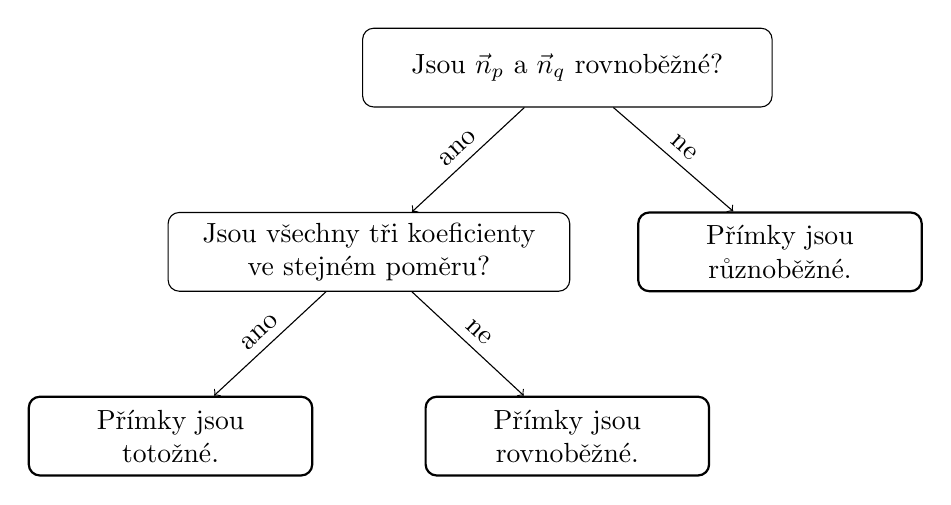
\begin{tikzpicture}[scale=0.9, every node/.style={align=center}]

        \node[draw, rounded corners, minimum width=5.2cm, minimum height=1cm]
            (start) at (0,0)
            {Jsou $\vec{n}_p$ a $\vec{n}_q$ rovnoběžné?};

        \node[draw, rounded corners, minimum width=5.1cm, minimum height=1cm]
            (coefficients) at (-2.8,-2.6)
            {Jsou všechny tři koeficienty\\ve stejném poměru?};

        \node[draw, rounded corners, minimum width=3.6cm, minimum height=1cm, thick]
            (intersecting) at (3,-2.6)
            {Přímky jsou\\různoběžné.};

        \node[draw, rounded corners, minimum width=3.6cm, minimum height=1cm, thick]
            (coincident) at (-5.6,-5.2)
            {Přímky jsou\\totožné.};

        \node[draw, rounded corners, minimum width=3.6cm, minimum height=1cm, thick]
            (parallel) at (0,-5.2)
            {Přímky jsou\\rovnoběžné.};

        \draw[->] (start) -- (coefficients)
            node[midway, above, sloped] {ano};
        \draw[->] (start) -- (intersecting)
            node[midway, above, sloped] {ne};
        \draw[->] (coefficients) -- (coincident)
            node[midway, above, sloped] {ano};
        \draw[->] (coefficients) -- (parallel)
            node[midway, above, sloped] {ne};

    \end{tikzpicture}
    \caption{Postup při určování vzájemné polohy přímek zadaných
    obecnými rovnicemi.}
    \label{fig:Relative_position_general_lines_decision}
\end{figure}

\paragraph{Rovnoběžné přímky}
\label{subsubsec:Parallel_general_lines}

Jsou-li normálové vektory dvou přímek rovnoběžné, mají přímky stejný
směr. Nejsou-li zároveň všechny tři koeficienty jejich obecných rovnic
ve stejném poměru, jde o dvě různé rovnoběžné přímky.

\begin{example}\label{exa:Parallel_general_lines}
    Určete vzájemnou polohu přímek $p:2x-3y+1=0$ a $q:-4x+6y+5=0$.
    
    Normálové vektory jsou
    \[
        \vec{n}_p=(2;-3),
        \qquad
        \vec{n}_q=(-4;6).
    \]
    Platí
    \[
        \vec{n}_q=-2\vec{n}_p,
    \]
    takže přímky mají stejný směr.

    Kdyby byly přímky totožné, musel by být stejným číslem $-2$
    vynásoben také absolutní člen. Platilo by tedy
    \[
        c_q=-2\cdot1=-2.
    \]
    Ve skutečnosti je však $c_q=5$. Všechny tři koeficienty proto
    nejsou ve stejném poměru a přímky jsou rovnoběžné:
    \[
        p\parallel q.
    \]
\end{example}

\begin{example}\label{exa:Parallel_general_line_through_point}
    Určete obecnou rovnici přímky $q$, která je rovnoběžná s přímkou $p:2x - 3y + 1 = 0$ a prochází bodem $K[-2;3]$.

    Rovnoběžná přímka může mít stejný normálový vektor
    \[
        \vec{n}_q=(2;-3).
    \]
    Její rovnice proto má tvar
    \[
        2x-3y+c=0.
    \]

    Dosadíme bod $K[-2;3]$:
    \begin{align*}
        2\cdot(-2)-3\cdot3+c&=0,\\
        -4-9+c&=0,\\
        c&=13.
    \end{align*}

    Hledaná přímka má rovnici
    \[
        q:2x-3y+13=0.
    \]
\end{example}

\paragraph{Různoběžné přímky a jejich průsečík}
\label{subsubsec:Intersecting_general_lines}

Nejsou-li normálové vektory dvou přímek rovnoběžné, mají přímky různé
směry a v rovině se protínají právě v jednom bodě. Souřadnice průsečíku
musí splňovat obě obecné rovnice současně, a proto je získáme řešením
soustavy těchto rovnic.

\begin{example}\label{exa:Intersecting_general_lines}
    Určete vzájemnou polohu přímek $p:2x+y-1=0$ a $q:x-y-2=0$.
    Jsou-li přímky různoběžné, určete jejich průsečík.

    Normálové vektory jsou
    \[
        \vec{n}_p=(2;1),
        \qquad
        \vec{n}_q=(1;-1).
    \]
    Tyto vektory nejsou rovnoběžné, protože neexistuje číslo $k$, pro
    které by platilo
    \[
        (1;-1)=k(2;1).
    \]
    Přímky jsou tedy různoběžné.

    Průsečík získáme řešením soustavy
    \begin{align*}
        2x+y-1&=0,\\
        x-y-2&=0.
    \end{align*}
    Po úpravě dostáváme
    \begin{align*}
        2x+y&=1,\\
        x-y&=2.
    \end{align*}

    Sečtením rovnic získáme
    \begin{align*}
        3x&=3,\\
        x&=1.
    \end{align*}
    Dosazením do druhé rovnice dostáváme
    \begin{align*}
        1-y&=2,\\
        y&=-1.
    \end{align*}

    Přímky se protínají v bodě
    \[
        P[1;-1],
    \]
    a proto
    \[
        p\cap q=\{P[1;-1]\}.
    \]
\end{example}

\paragraph{Totožné přímky}
\label{subsubsec:Coincident_general_lines}

Jsou-li všechny tři koeficienty jedné obecné rovnice stejným
nenulovým násobkem koeficientů druhé rovnice, popisují obě rovnice
tutéž množinu bodů. Přímky jsou proto totožné.

\begin{example}\label{exa:Coincident_general_lines}
    Určete vzájemnou polohu přímek $p:2x-3y+1=0$ a $q:-4x+6y-2=0$.

    Pro vektory platí
    \[
        (2;-3) = -\frac{1}{2}(-4;6)
    \]
    Z toho je zřejmé, že přímky jsou buď rovnoběžné anebo totožné.
    Zjistíme, zdali bod z přímky $p$ náleží přímce $q$. Najdemte tedy bod ležící na přímce $p$,
    tak že dosadíme jednu libovolnou souřadnici, např $x = -2$ a druhou dopočítáme. 

    \begin{align*}
        2 \cdot (-2) - 3y + 1 &= 0, \\
        -4 -3y +1 &= 0, \\
        -3y &= 3, \\
        y &= -1.
    \end{align*}

    Bod ležící na přímce $p$ je tedy $P[-2;-1]$. A ověříme zdali tento bod leží i na přímce $q$.

    \begin{align*}
        -4 \cdot (-2) + 6 \cdot (-1) - 2 &= 0, \\
        8 - 6 - 2 &= 0, \\
        0 &= 0.
    \end{align*}

    Protože bod $P[-2;-1]$ náleží oběma přímkám a zároveň jejich normálové vektory jsou rovnoběžné,
    pak jsou přímky totožné.

    Další způsob řešení je využítím toho, že pro koeficienty platí
    \[
        (-4;6;-2)=-2(2;-3;1).
    \]
    Druhá rovnice tedy vznikla vynásobením první rovnice číslem $-2$.
    Obě rovnice mají stejnou množinu řešení, a proto jsou přímky
    totožné:
    \[
        p=q.
    \]
    Jejich průnikem je celá přímka:
    \[
        p\cap q=p=q.
    \]
\end{example}

\paragraph{Kolmé přímky}
\label{subsubsec:Perpendicular_general_lines}

Dvě přímky jsou kolmé právě tehdy, když jsou kolmé jejich směrové
vektory. Protože pootočením obou vektorů o $90^\circ$ se velikost úhlu
mezi nimi nezmění, můžeme kolmost ověřovat také pomocí normálových
vektorů.

Pro přímky
\[
    p:a_1x+b_1y+c_1=0
\]
a
\[
    q:a_2x+b_2y+c_2=0
\]
platí
\begin{equation}\label{eq:Perpendicular_general_lines}
    p\perp q
    \quad\Longleftrightarrow\quad
    a_1a_2+b_1b_2=0.
\end{equation}

\begin{example}\label{exa:Perpendicular_general_lines}
    Určete vzájemnou polohu přímek
    \[
        p:x+2y-5=0
    \]
    a
    \[
        q:2x-y-5=0.
    \]

    Normálové vektory jsou
    \[
        \vec{n}_p=(1;2),
        \qquad
        \vec{n}_q=(2;-1).
    \]
    Jejich skalární součin je
    \[
        \vec{n}_p\cdot\vec{n}_q
        =
        1\cdot2+2\cdot(-1)
        =
        0.
    \]
    Přímky jsou proto kolmé:
    \[
        p\perp q.
    \]

    Jejich průsečík získáme řešením soustavy
    \begin{align*}
        x+2y&=5,\\
        2x-y&=5.
    \end{align*}
    Z druhé rovnice vyjádříme
    \[
        y=2x-5
    \]
    a dosadíme do první:
    \begin{align*}
        x+2(2x-5)&=5,\\
        5x-10&=5,\\
        x&=3.
    \end{align*}
    Potom
    \[
        y=2\cdot3-5=1.
    \]
    Kolmé přímky se protínají v bodě
    \[
        P[3;1].
    \]
\end{example}

\begin{example}\label{exa:Perpendicular_general_line_through_point}
    Určete obecnou rovnici přímky $q$, která je kolmá k přímce $p:2x-3y+1=0$ a prochází bodem $K[-2;3]$.
    
    Normálový vektor přímky $p$ je
    \[
        \vec{n}_p=(2;-3).
    \]
    Směrový vektor přímky $p$ můžeme zvolit například
    \[
        \vec{u}_p=(3;2).
    \]

    Hledaná přímka $q$ má být k přímce $p$ kolmá. Její normálový vektor
    proto může být rovnoběžný se směrovým vektorem přímky $p$. Zvolíme
    \[
        \vec{n}_q=(3;2).
    \]

    Rovnice hledané přímky má tvar
    \[
        3x+2y+c=0.
    \]
    Dosadíme bod $K[-2;3]$:
    \begin{align*}
        3\cdot(-2)+2\cdot3+c&=0,\\
        -6+6+c&=0,\\
        c&=0.
    \end{align*}

    Hledaná kolmice má rovnici
    \[
        q:3x+2y=0.
    \]
\end{example}

\begin{example}\label{exa:Central_symmetry_line}
    Je dána přímka
    \[
        p:2x-y+1=0.
    \]
    Určete rovnici přímky $p'$, která je obrazem přímky $p$ ve
    středové souměrnosti se středem
    \[
        S[-2;1].
    \]

    Přímku $p'$ můžeme určit pomocí obrazů dvou různých bodů přímky
    $p$. Pro obraz libovolného bodu $X$ ve středové souměrnosti se
    středem $S$ platí
    \[
        X'=S+(S-X)=2S-X.
    \]

    Nejprve tedy na přímce $p$ zvolíme dva různé body, určíme jejich
    obrazy a následně sestavíme rovnici přímky procházející těmito
    obrazy.

    Zvolíme nejprve bod s první souřadnicí $x=0$. Dosadíme do rovnice
    přímky $p$:
    \begin{align*}
        2\cdot0-y+1&=0,\\
        -y+1&=0,\\
        y&=1.
    \end{align*}

    Na přímce $p$ tedy leží bod
    \[
        A[0;1].
    \]

    Jako druhý bod zvolíme bod s první souřadnicí $x=1$:
    \begin{align*}
        2\cdot1-y+1&=0,\\
        3-y&=0,\\
        y&=3.
    \end{align*}

    Druhým bodem přímky $p$ je
    \[
        B[1;3].
    \]

    Nyní určíme obraz bodu $A$ ve středové souměrnosti se středem
    $S[-2;1]$:
    \begin{align*}
        A'
        &=
        S+(S-A)\\
        &=
        [-2;1]+\bigl([-2;1]-[0;1]\bigr)\\
        &=
        [-2;1]+(-2;0)\\
        &=
        [-4;1].
    \end{align*}

    Obdobně určíme obraz bodu $B$:
    \begin{align*}
        B'
        &=
        S+(S-B)\\
        &=
        [-2;1]+\bigl([-2;1]-[1;3]\bigr)\\
        &=
        [-2;1]+(-3;-2)\\
        &=
        [-5;-1].
    \end{align*}

    Obrazem přímky $p$ je přímka $p'$, která prochází body
    \[
        A'[-4;1]
        \qquad\text{a}\qquad
        B'[-5;-1].
    \]

    Její směrový vektor můžeme určit jako
    \[
        \overrightarrow{A'B'}
        =
        (-5-(-4);-1-1)
        =
        (-1;-2).
    \]

    K tomuto směrovému vektoru zvolíme normálový vektor
    \[
        \vec{n}_{p'}=(2;-1),
    \]
    protože
    \[
        (-1;-2)\cdot(2;-1)
        =
        -2+2
        =
        0.
    \]

    Obecná rovnice přímky $p'$ má tedy tvar
    \[
        2x-y+c=0.
    \]

    Dosadíme například bod $A'[-4;1]$:
    \begin{align*}
        2\cdot(-4)-1+c&=0,\\
        -8-1+c&=0,\\
        c&=9.
    \end{align*}

    Hledaná přímka má rovnici
    \[
        p':2x-y+9=0.
    \]

    Přímky $p$ a $p'$ mají stejné normálové vektory, a jsou proto
    rovnoběžné. To odpovídá vlastnosti středové souměrnosti: obrazem
    přímky, která neprochází středem souměrnosti, je přímka s ní
    rovnoběžná.

    \begin{figure}[H]
        \centering
        \begin{tikzpicture}[scale=0.9]

            % Přímky
            \draw[thin, <->]
                (-1.5,-2) -- (2.5,6)
                node[above right] {$p$};

            \draw[thin, <->]
                (-5.5,-2) -- (-1.5,6)
                node[above right] {$p'$};

            % Body
            \coordinate (A) at (0,1);
            \coordinate (B) at (1,3);
            \coordinate (S) at (-2,1);
            \coordinate (Ap) at (-4,1);
            \coordinate (Bp) at (-5,-1);

            \fill (A) circle (2.5pt)
                node[below right] {$A$};
            \fill (B) circle (2.5pt)
                node[below right] {$B$};
            \fill (S) circle (2.5pt)
                node[above right] {$S$};
            \fill (Ap) circle (2.5pt)
                node[above left] {$A'$};
            \fill (Bp) circle (2.5pt)
                node[below left] {$B'$};

            % Spojnice bodů se středem
            \draw[vector] (A) -- (S);
            \draw[vector] (S) -- (Ap);

            \draw[vector] (B) -- (S);
            \draw[vector] (S) -- (Bp);

        \end{tikzpicture}
        \caption{Přímka $p'$ je obrazem přímky $p$ ve středové
        souměrnosti se středem $S$.}
        \label{fig:Central_symmetry_line}
    \end{figure}
\end{example}